% !TeX root = ../main.tex

\chapter{性能分析与优化(安全性与稳定性分析)}

\section{测试平台}
由于AOSP仅源码就有130G之多,在完成编译之后达到212G,因此构建Android镜像需要一台性能充足构建机以及用于烧录运行镜像的测试机。
构建机需要充足的存储空间以及编译大量内容,所以选择核数多性能强的服务器,测试机是目标系统镜像的运行平台。

\textbf{构建机}:在构建安卓内核、镜像,以及编译loonggpu核模块都使用的是龙芯公司的X86服务器(所有模块都是交叉编译),Xeon Gold 6388处理器,核数为128核。

\textbf{构建环境配置}:

    AOSP镜像构建:AOSP配置环境使用预先编译好的llvm15的编译器(这些前期已完成),通过AOSP项目提供的envsetup.sh脚本设置基本的环境变量,并lunch loongarch-3A5000选择构建目标,
        设置特有的环境变量。编译上可以选择使用m编译全平台代码,mm编译某模块代码及其依赖或者使用mmm编译某个指定路径下的所有路径及其依赖。

    Android内核构建:编译工具链使用loongson\ gnu\ toolchain 8.3,使用自写脚本设置交叉编译环境变量,主要是PATH、LD\_LIBRARY\_PATH、CROSS\_COMPILE、ARCH等变量的指定,
        最后使用make编译,可以使用-j(\$proc)添加编译核心数。

    核模块构建:构建与内核编译类似,设置交叉编译环境后使用make即可编译。

\textbf{测试机}:运行主机是LoongArch64结构,使用龙芯的3A5000CPU,配备7A2000桥片。桥片上集成了LG110显卡,该显卡所使用的固件需要在Android内核构建时以被编入,而内核驱动在安卓系统进入shell时
    通过insmod(/rmmod)加载(或删除)该模块。

\section{测试内容}

\subsection{功能测试}
由于本课题是从内核重新搭建整个图形栈,所以从底向上依次内核驱动测试、libdrm测试、gralloc和hwcomposer测试,最后渲染引擎测试和SurfaceFlinger测试。

\textbf{内核驱动测试}:由于是设备模块驱动的测试,需要通过内核的debugfs进行测试,mount -t debugfs none debug挂载debug文件系统,对LG110的3个环形缓冲区进行测试,分别是
ib、gfx、xdma,通过所有测试用例\ref{fig:内核驱动测试结果}

\begin{figure}[h]
    \centering
    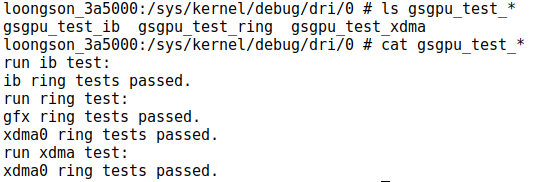
\includegraphics[width=0.8\textwidth]{内核驱动测试结果.png}
    \caption{内核驱动测试结果}
    \label{fig:内核驱动测试结果}
\end{figure}

\textbf{libdrm正确性测试}
libdrm中有关LG110的测试共有5个测试套件,使用Cunit单元测试框架编写如\ref{tab:libdrm_gsgpu测试集}。其中:

basic\_tests是GPU基础功能测试集,包含测试查询GPU信息的功能、用户空间内存访问功能、缓冲区的逐出功能、GPU 命令提交的功能、多栅栏同步功能 、信号量功能共6部分。

bo\_tests是缓冲区对象功能测试集,包括缓冲区对象导入导出、缓冲区对象映射解映射、缓冲区对象的元数据处理功能、规范显卡内存分配、不规范显卡内存分配共5部分。

dma\_tests是DMA相关功能的测试集,包括DMA线性写、DMA常量填充、DMA线性拷贝测试、DMA Tiled拷贝测试、MSAA(多重采样抗锯齿)图像测试、Mipmap(多级渐远纹理)生成测试、
DMA信号量处理测试共7例测试用例。

deadlock\_tests是死锁测试集,测试GFX环和DMA环是否会发生死锁共两例。

vm\_tests是虚拟内存ID测试集,测试了虚拟内存ID(VMID)预留机制共一例。

共21例测试用例全部通过测试。

\begin{table}[h]
    \centering
    \caption{libdrm\_gsgpu测试集}
    \label{tab:libdrm_gsgpu测试集}
    \begin{tabular}{lll}
      \toprule
      类名   &  数量  &通过数量\\
      \midrule
      basic\_tests & 6 & 6\\
      bo\_tests & 5 & 5\\
      dma\_tests & 7 & 7\\
      deadlock\_tests & 2 &2\\
      vm\_tests & 1 &1\\
      \bottomrule
    \end{tabular}
    \note{}
\end{table}

\textbf{gralloc测试}
gralloc功能测试采纳了两部分,一是谷歌官方提供的原生测试用例,是AOSP中framework(框架代码)提供的gralloc测试用例GrallocTypes\_test,
其主要是使用GTest编写。
GTest\cite{GoogleTest}是由 Google 开发的一款 C++ 测试框架,用于编写单元测试。它广泛应用于软件开发中,帮助开发人员验证代码的正确性,检测潜在的错误和缺陷。
另一部分是gralloc0的测试用例(gralloc0主要存在于Android OREO版本之前),主要涵盖了一些基本的图形缓冲区的测试等。
gralloc0 是Android较早的图形内存管理接口,通常与较老的硬件和系统版本一起使用,gralloc4是在gralloc0的基础上进行功能拓展,因此使用gralloc0的测试用例不仅可以测试gralloc的基础功能,
还可以测试gralloc模块对于较老硬件和系统的兼容性。

GrallocTypes\_test主要是用来验证Android12 系统中 Gralloc4 的功能,确保与图形缓冲区相关的各种数据类型(如像素格式、压缩、元数据等)
能够正确地序列化和反序列化。测试用例涵盖了广泛的输入类型,确保编码和解码过程能够正确工作,同时处理标准类型和扩展类型。
经测试,已通过全部的21个测试套件共180个测试用例,如图\ref{fig:GrallocTypeGtest测试图},测试结果过长仅做部分截图。

\begin{figure}[h]
    \centering
    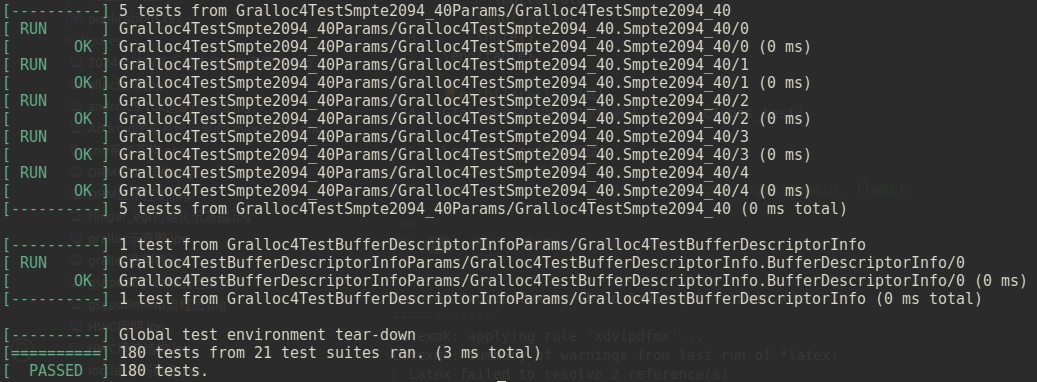
\includegraphics[width=0.8\textwidth]{GrallocTypeGtest测试图.png}
    \caption{GrallocTypeGtest测试图}
    \label{fig:GrallocTypeGtest测试图}
\end{figure}

gralloc0测试用例,主要测试了内存缓冲区的分配与释放、图形缓冲区锁定与解锁、API版本的兼容性以及性能和行为测试,如\ref{tab:gralloc0测试集}。

\begin{table}[h]
    \centering
    \caption{gralloc0测试集}
    \label{tab:gralloc0测试集}
    \begin{tabular}{lll}
      \toprule
      测试项   &  描述 & 结果 \\
      \midrule
      test\_alloc\_varying\_sizes & 测试不同尺寸缓冲区的分配和释放 & passed\\
      test\_alloc\_combinations & 测试多种格式和用途组合的缓冲区分配 & passed\\
      test\_api & 测试 gralloc 模块的API版本,验证支持的功能 & passed\\
      test\_gralloc\_order & 测试缓冲区注册、注销、锁定和解锁操作的顺序 & passed\\
      test\_mapping & 测试CPU对内存的读取和写入 & passed\\
      test\_perform & 测试一些私有API操作,如获取缓冲区的额外信息等 & passed\\
      test\_ycbcr & 测试YUV格式的缓冲区的锁定操作 & passed\\
      test\_async & 测试异步锁定和解锁 & passed\\
      \bottomrule
    \end{tabular}
    \note{}
\end{table}

\textbf{hwcomposer测试}
hwcomposer由于分为客户端和服务端,所以有关客户端的测试用例主要存在于framework下的SurfaceFlinger的实现源码中的CompositionEngine目录下,
主要用于测试CompositionEngine调用hwcomposer的实现是否正确。

Composition测试
hwc测试

\textbf{渲染引擎测试}
librenderengine\_test也是AOSP中提供的安卓原生测试用例,分为两部分一部分是渲染管线测试(验证RenderEngine模块在不同场景下的正确性,确保图形层、颜色、阴影以及变换等操作正常工作)
以及渲染线程测试(验证RenderEngineThreaded在多线程环境下是否正确代理调用、处理异步操作及状态同步)2个测试套件例共295个测试用例,包括渲染固体颜色、缓冲区变换、Alpha混合行为、
渲染带阴影的图层、使用不同的变换和裁剪渲染图层、色彩空间中的颜色管理、纹理测试、线程安全的属性传递、多线程同步处理等多种异常情况,较为全面,可通过全部的295个测试用例。

% \begin{figure}[h]
%     \centering
%     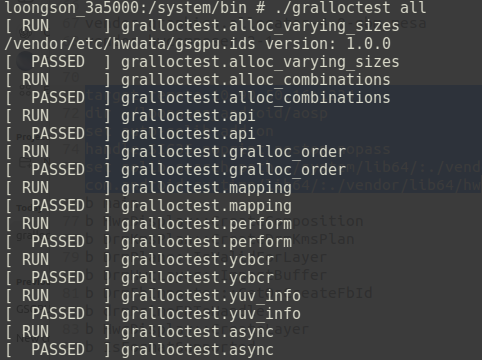
\includegraphics[width=0.8\textwidth]{gralloc0测试截图.png}
%     \caption{gralloc0测试截图}
%     \label{fig:gralloc0测试截图}
% \end{figure}

\textbf{SurfaceFlinger测试}
对SurfaceFlinger的测试包含两个部分,一个是SurfaceFlinger的单元测试libsurfaceflinger\_unittest,另一个是SurfaceFlinger\_test。


\subsection{性能测试}
% bocreate 缓冲重用
% pb_cache_bucket = gsgpu_get_heap_index(domain, flags);

% \section{启动时间优化}

% \section{PAGE\_SIZE调整带来的影响评估}

% \section{性能分析}

% \section{兼容性测试}

% \subsection{surfaceflinger关键流程分析}

% \subsection{性能分析软硬件环境和方法} gtestopengl 测试套件

% \subsection{结论}

% \section{???}

